\chapter{Design and fabrication}\label{ch:design}

In this chapter, the elements of wind tunnel, the design dimensions and its calculations with respect to the solid cylinder are discussed.
\section{Elements of the Wind Tunnel Setup:}

\begin{enumerate}

\item Test Section: In the test section, a solid cylinder is placed at the center to induce vortex shedding. As air flows past the cylinder, it generates a turbulent wake leading to vortex formations, which needs to be studied to understand the dynamics of fluid flow and the effects of varying conditions such as flow velocity (Reynolds number).

\item Flow Control (Exhaust Fan or Suction Fan): The air flow through the wind tunnel is generated by an exhaust fan that creates a continuous flow of air. This suction fan is integrated into the system to help maintain a consistent air velocity by drawing air through the tunnel, ensuring steady and controlled flow conditions for the experiments.

\item Hot-Wire Anemometer: The hot wire anemometer in this set-up is directly connected to a constant current DC source and an oscilloscope. The DC source provides a steady current to the hot wire, which heats up as the current passes through it. As air passes through the wire, it cools the wire, causing a change in its electrical resistance. These changes in resistance are captured by the oscilloscope, allowing real-time monitoring of the airflow velocity. The oscilloscope displays the voltage fluctuations, which correspond to variations in airspeed, providing detailed data for analyzing vortex-shedding behavior and other characteristics of fluid dynamics.

\end{enumerate}
The wind tunnel is designed with a square cross section, providing adequate space for the cylindrical test object and allowing air flow to develop uniformly before reaching the test section. The dimensions of the tunnel are chosen to ensure a stable and controlled environment for accurate experimentation.


\section{Main parts of the wind tunnel:}

This section discusses the main parts of the wind tunnel. Each part serves a specific purpose, such as improving flow quality, controlling velocity, or ensuring stable air flow to and from the test section. Fig.~\ref{fig:wind_tunnel} shows the basic wind tunnel test rig used in this project. There are certain assumptions made, which are given below:

\begin{figure}[h]
    \centering
    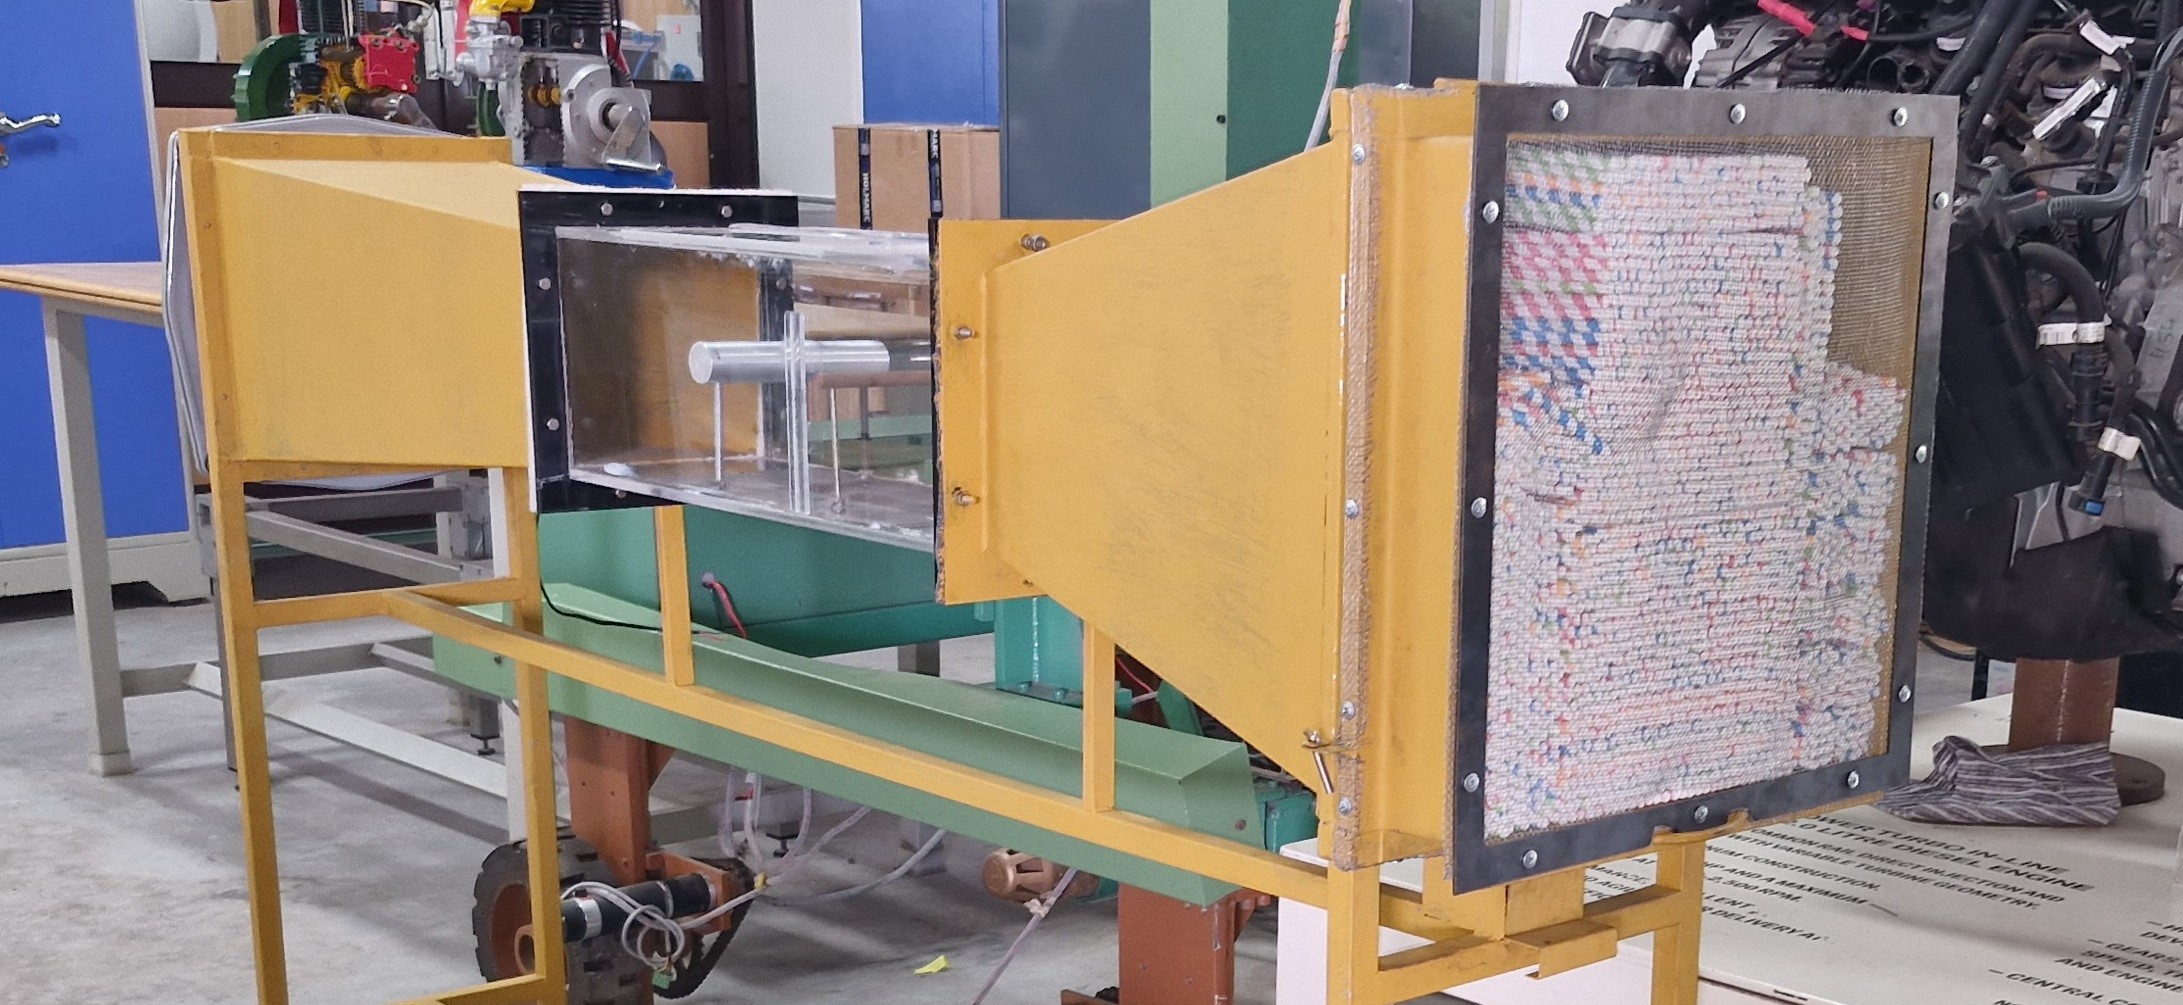
\includegraphics[width=0.9\linewidth]{gfx/windtunnel.jpg}
    \caption{Wind tunnel test rig.}
    \label{fig:wind_tunnel}
\end{figure}

\begin{itemize}

\item The air flows in the subsonic region and is incompressible.

\item The tunnel is assumed to be steady, with a uniform flow before the cylinder.

\item The Reynolds number will be chosen on the basis of typical flow conditions in the wind tunnel.

\end{itemize}
The following sections discuss the parts of the wind tunnel.
\subsection{Settling chamber}

The settling chamber is the first section of the wind tunnel. Its primary purpose is to stabilize the air flow and remove large turbulence before the air moves into the contraction section.

% \subsubsection{Purpose:}
% \begin{itemize}
% \item Reduce large-scale turbulence.

% \item Allow airflow to become more uniform and laminar before entering the contraction section.
% \end{itemize}
\subsubsection{Length calculations:}

The length of the settling chamber is usually between 0.25 to 4 times the width of the tunnel.  Width of the settling chamber (W$_{\text{settling}}$) is taken as 0.4 m. The length of the settling chamber (L$_{\text{settling}}$) should be between 0.1 m and 0.15 m and it is taken as 0.1 m  for better flow conditioning.


\subsection{Contraction Section}
The contraction section is used to accelerate the flow towards the test section while ensuring that the air flow remains smooth. This section converges the cross-sectional area, accelerating the air and increasing the velocity as it moves through the wind tunnel.
\begin{figure}[H]
    \centering
    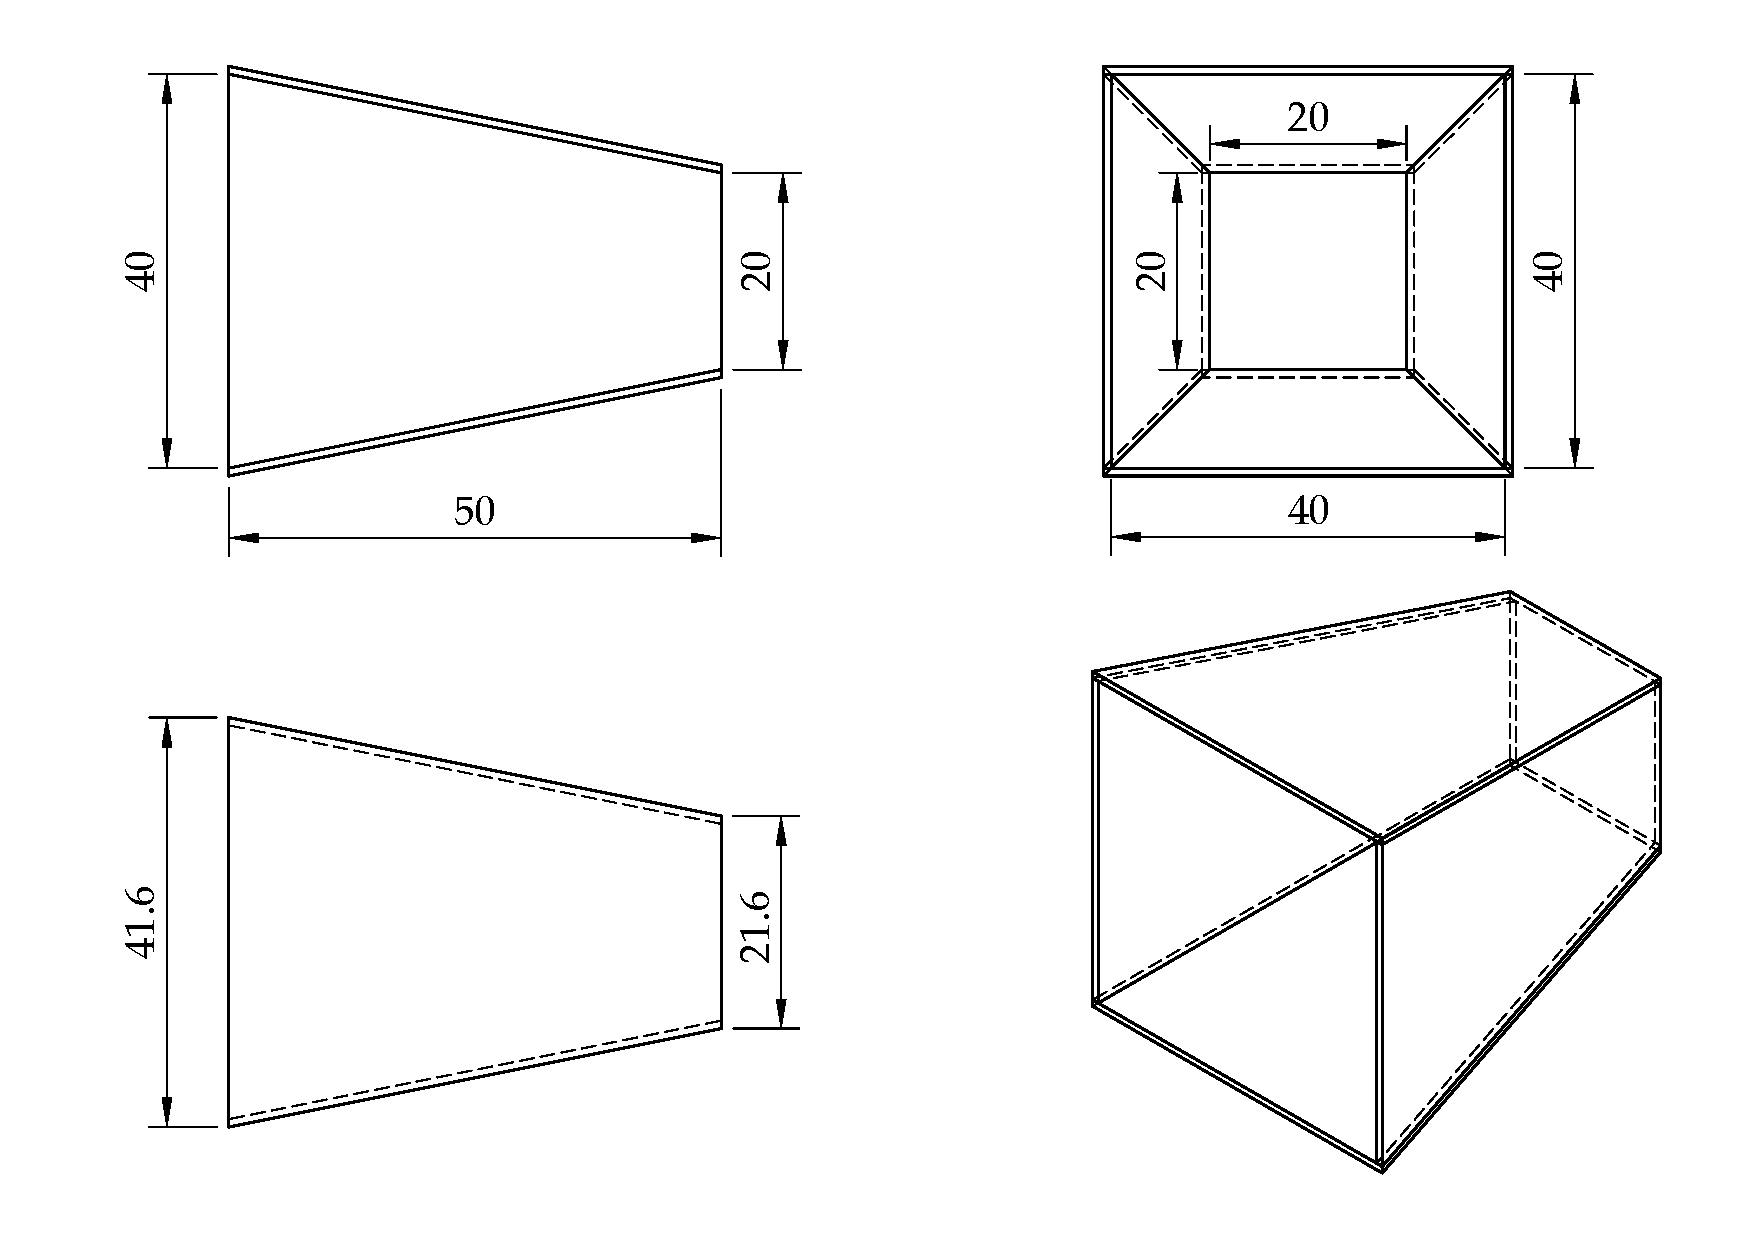
\includegraphics[width=\linewidth]{gfx/Convergent_section_wind_tunnel.pdf}
    \caption{Dimensions of converging section.}
    \label{fig:converge section}
\end{figure}

% \subsubsection{Purpose:}
% \begin{itemize}

% \item To accelerate the flow towards the test section.

% \item To ensure that the flow remains laminar and does not separate.
% \end{itemize}
%\subsubsection{Design parameters}
%\begin{itemize}

%\end{itemize}
\subsubsection{Design Parameters}
A typical contraction ratio (the ratio between the cross-sectional area of the inlet and the cross-sectional area of the test section) is 4:1 for laminar flow. This ensures that the air accelerates smoothly as it enters the test section. The height of the contraction section, H$_{\text{Contraction}}$ = 20 cm and the width of the contraction section, W$_{\text{Contraction}}$ = 20 cm. The length of the contraction section is typically 2 to 5 times the width of the test section. So, length of the contraction section, L$_{\text{Contraction}}$ = 0.5 m 
%\end{itemize}

\subsection{Test Section}
The object (solid cylinder) is placed in the test section and the vortex shedding and flow measurements are analyzed. The air flow for analysis should be uniform. The test section provides uniform airflow for analysis. The calibration of the bulb filament and the hot wire anemometer is performed in the test section. Vortex analysis is also performed in the test section.

\begin{figure}[H]
    \centering
    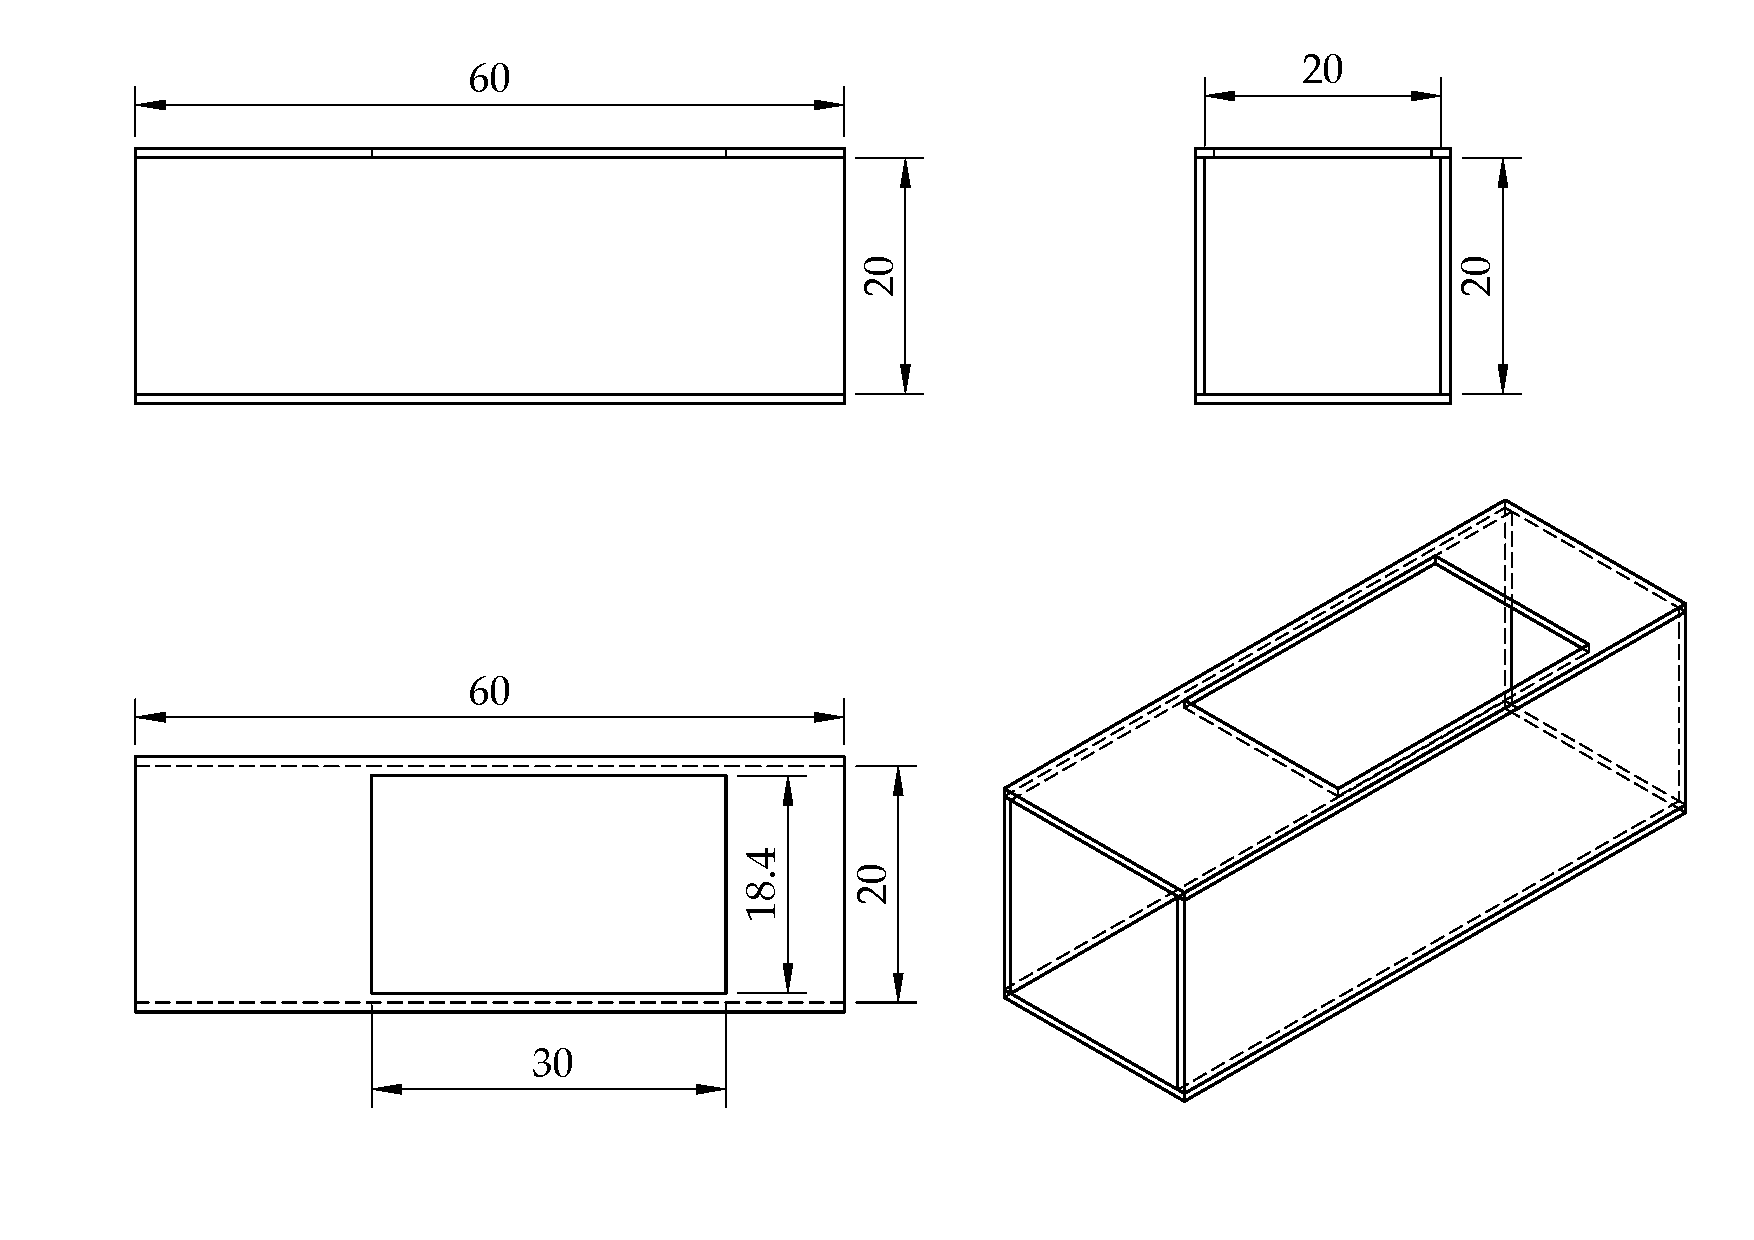
\includegraphics[width=\linewidth]{gfx/Wind_tunnel_test_section.pdf}
    \caption{Dimensions of the test section.}
    \label{fig:test section}
\end{figure}
%\subsubsection{Purpose:}
% \begin{itemize} 

% \item 

% \item Measure velocity changes with the tungsten bulb filament and hot wire anemometer.
% \end{itemize}
\subsubsection{Design parameters:}
%\begin{itemize}
The width and height of the test section should be at least 5–10 times the diameter of the cylinder. The diameter of the D-cylinder is 0.033 m (33 mm). So width and height of the test section is 
\begin{align}
W_{\text{test}} = 7 \times D = 7 \times\ 0.033 = 0.23 m\label{width test section}, \\
H_{\text{test}} = 7 \times D = 7 \times 0.033 = 0.23 m \label{height test section}.
\end{align}
So, the test section is designed to have a square cross section of side having 20~cm length.
%\end{itemize}
%\subsubsection{Length calculation:}
The length of the test section should be long enough to allow a fully developed flow before the air flow reaches the cylinder. The length is typically between 10 to 20 times the diameter of the test object (the cylinder) to allow for stable flow development. So, the length of the test section,
\begin{align}\label{length test section}
L_{\text{test}} = 18 \times D = 18 \times 0.033 =  0.6 m
\end{align}

\subsection{Diffuser Section}
The Diffuser Section is the final section of the wind tunnel, and its purpose is to slow down the airflow after the test section while minimizing turbulence. In this section, the airflow expands in the cross-sectional area, leading to a decrease in the velocity of the air, which helps to prevent any damage or instability in downstream equipment such as fans or flow measurement instruments. In addition, the diffuser allows the pressure to recover smoothly. The diffuser should have a gentle expansion to avoid turbulent separation. The cross-sectional area of the diffuser gradually increases, which reduces the velocity of the flow. The expansion ratio (the ratio of the inlet to the outlet area) is typically between 1.5:1 to 2:1 to ensure smooth deceleration without flow separation.
\begin{figure}[H]
    \centering
    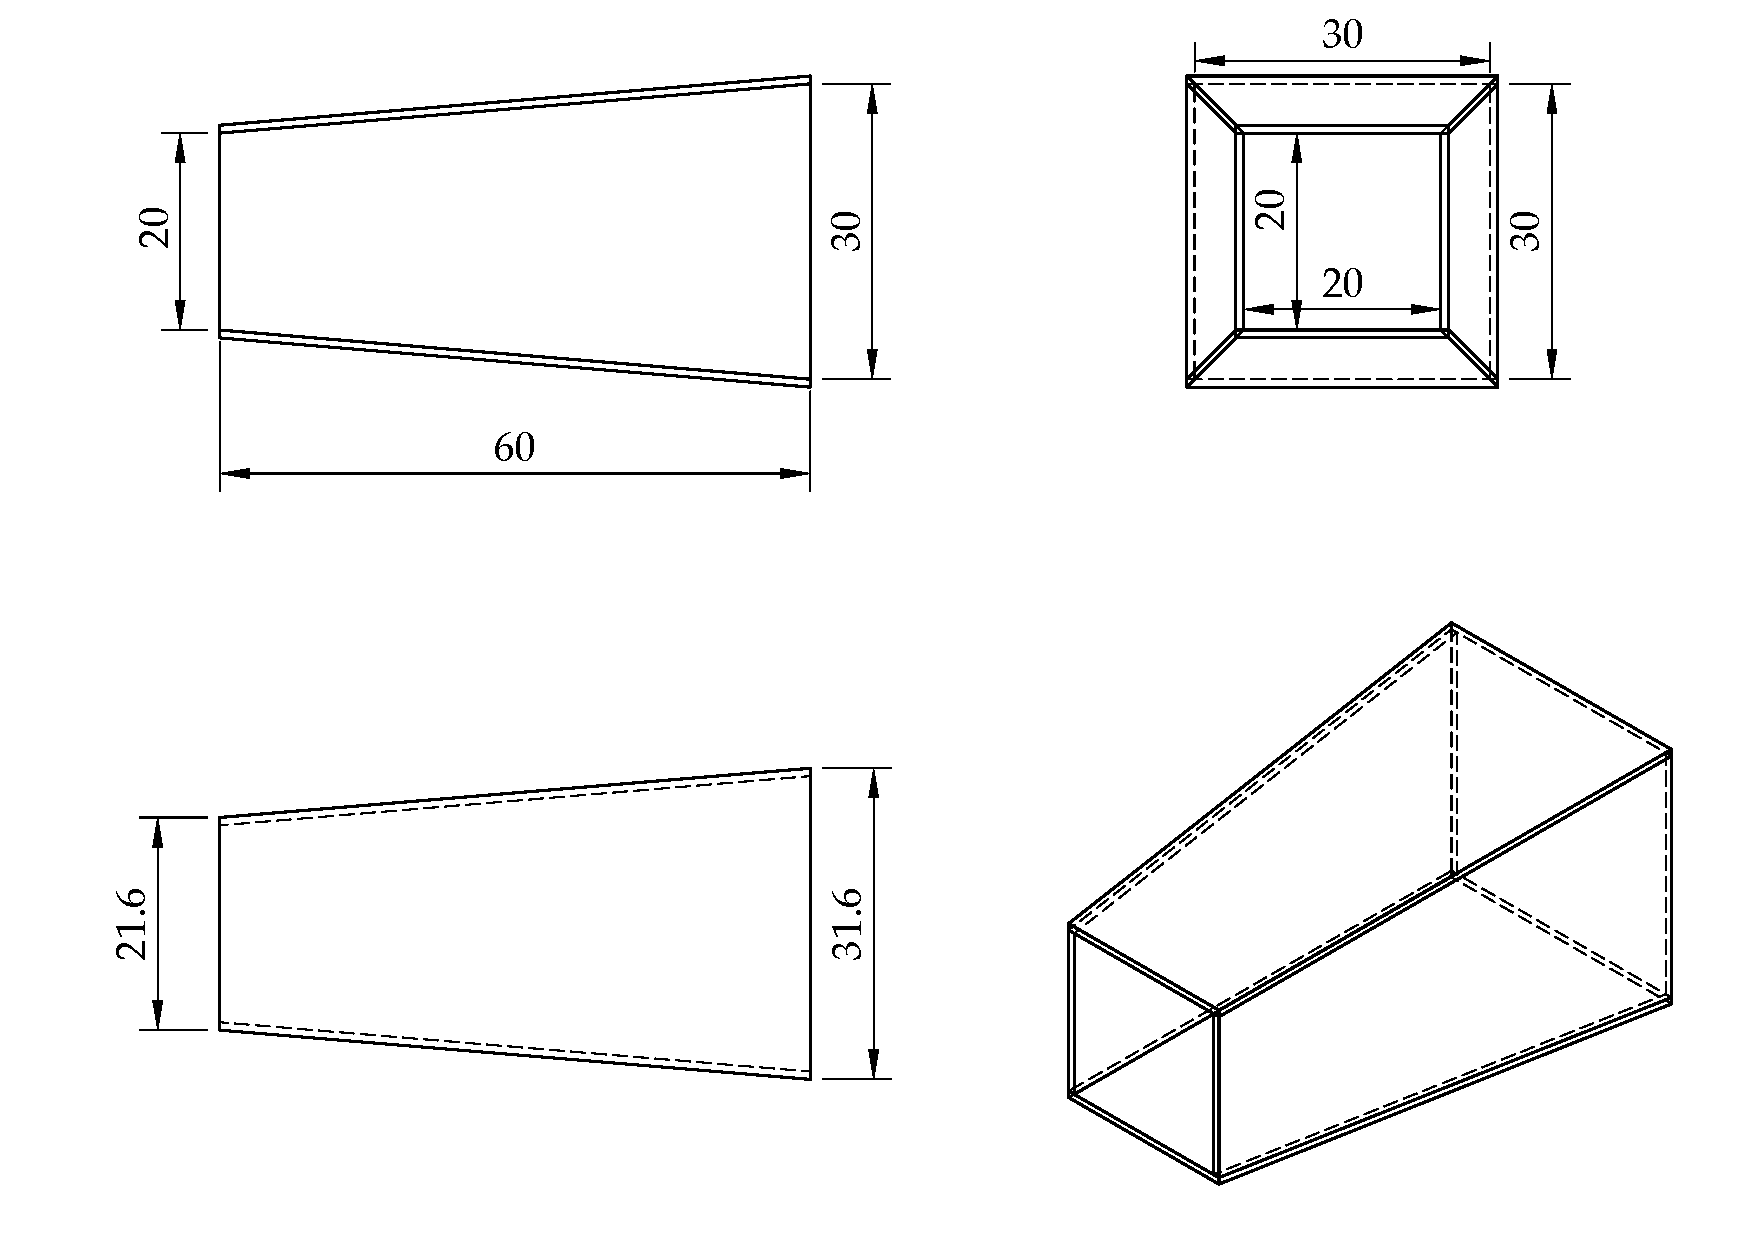
\includegraphics[width=\linewidth]{gfx/Divergent_section_for_wind_tunnel.pdf}
    \caption{Dimensions of diverging section.}
    \label{fig:diverge section}
\end{figure}
\subsubsection{Design parameters}
%The width and height of the diffuser section is designed in such a way that it expands relative to the test section.
The diffuser must also allow for the transition from the uniform flow of the test section to the slower flow at the exit of the tunnel. The cross section of the diffuser section near the test section should be equal to the cross section of the test section. It should gradually increase at the other end for smooth flow expansion.
%Since the width and height of the test section are decided to be 0.2 m, the diffuser section can be designed with the following dimensions:
So, the width (W$_{\text{diffuser}}$) and height (H${_\text{diffuser}}$) of the diffuser near the test section is 0.2~m and it is 0.4~m at the end. 
%Increase the width gradually from 0.2 m to a higher value, ensuring a smooth transition. Typically, the width may expand to 0.3 m at the end of the diffuser.
%Height : The height should also increase from 0.2 to 0.3 m, maintaining the ratio of the test section.Height of diffuser section = 0.3 m

Length of the diffuser should be long enough to allow the flow to gradually decelerate and the pressure to recover smoothly. The length is generally 2 to 5 times the width of the diffuser section. Since the diffuser width at the end is 0.3 m, the length of the diffuser is
\begin{align}
    L_{\text{Diffuser}}= 2 \times 0.3 = 0.6~m\nonumber
\end{align}
% L$_{\text{Diffuser section}}$ = 2 × W$_{\text{Diffuser section}}$ to 5 × w$_{\text{Diffuser section}}$

% Substituting the width:

% Length of diffuser section,

To design a gentle expansion, the ratio of the inlet area (of the test section) to the outlet area (of the diffuser) should be between 1.5:1 to 2:1. This would allow the air to decelerate without excessive turbulence.

\section{Hot Wire Filament}

When selecting a hot wire filament that is used in light bulbs or heating elements, it is essential to calculate its resistance, surface area and the maximum temperature at which the filament can operate safely. Below is a detailed breakdown of how to select the filament based on the provided information: The resistance of the filament and the operating temperature are calculated on the basis of material properties and filament dimensions. The resistance $R$ of the filament can be estimated using the equation
\begin{equation}\label{eq:resistance}
R = \rho_w \frac{L_w}{A_w},
\end{equation}
where $\rho_w$ is the resistivity of tungsten ($5.6 \times 10^{-8}\Omega m$), $L_w$ is the length of the filament ($4~mm$) and $A_w$ is the cross-sectional area of the filament ($7.853 \times 10^{-12}~m^2$). 
%calculated using the diameter \( d = 0.1 \, mm = 0.1 \times 10^{-3} \, m \).
Substituting the values in Eq.~(\ref{eq:resistance}), the resistance $R$ of the filament is estimated to be $0.03\Omega$. The maximum operating temperature of the filament is determined using the energy balance equation
\begin{equation}\label{eq:energy balance}
I^2 R = h A_w (T_{\text{wire}} - T),    
\end{equation}
where $I$ is the current, $R$ is the resistance of the wire (Eq.~(\ref{eq:resistance})), $h$ is the heat transfer coefficient ($10~W/m^2K$), $A$ is the surface area of the filament ($1.256 \times 10^{-5}~m^2$) and $T$ is the ambient temperature ($32^\circ C$). Substituting the above values in Eq.~(\ref{eq:energy balance}), the maximum filament temperature $T_{\text{wire}}$ can be estimated to be $300^\circ C$. Thus, the tungsten filament will operate at a maximum temperature of approximately 300 ° C.

% \section*{Design Parameters}
% \begin{itemize}
%     \item \textbf{Material}: Tungsten
%     \item \textbf{Filament Length}: 4 mm
%     \item \textbf{Filament Diameter}: 0.1 mm
%     \item \textbf{Resistance}: 0.03 $\Omega$
%     \item \textbf{Cross-sectional Area}: \( 7.853 \times 10^{-12} \, \text{m}^2 \)
%     \item \textbf{Surface Area}: \( 1.256 \times 10^{-5} \, \text{m}^2 \)
%     \item \textbf{Ambient Temperature}: 32 °C
%     \item \textbf{Maximum Filament Temperature}: 300 °C
% \end{itemize}


\section{Fan Power calculation}
This section provides a detailed calculation to determine the required fan power for a wind tunnel with the dimensions described in the previous section and the flow conditions. 
%The calculations include the area, velocity, pressure drop across various sections and the final fan power required to maintain a test section velocity of 20 m/s.

\subsection{Area Calculations}
%The cross-sectional area of each section is calculated as
Area of the contraction section
\begin{equation}\label{area of contraction}
A_{\text{contraction}} = W_{\text{contraction}}\cdot H_{\text{contraction}} = 0.4\cdot 0.4 = 0.16~\text{m$^2$},
\end{equation}
area of the test section
\begin{equation}\label{area of test}
    A_{\text{test}} = W_{\text{test}}\cdot H_{\text{test}} = 0.2\cdot 0.2 = 0.04~\text{m$^2$}
\end{equation}  
and the area of the diffuser section
\begin{equation}\label{area of diffuser}
    A_{\text{diffuser}} = W_{\text{diffuser}} \cdot H_{\text{diffuser}} = 0.3 \cdot 0.3 = 0.09 ~\text{m}^2.
\end{equation}


% \begin{align}
% A_{\text{settling}} &= W_{\text{settling}} \cdot H_{\text{settling}} = 0.4 \, \text{m} \cdot 0.4 \, \text{m} = 0.16 \, \text{m}^2. \\
% A_{\text{test}} &= W_{\text{test}} \cdot H_{\text{test}} = 0.2 \, \text{m} \cdot 0.2 \, \text{m} = 0.04 \, \text{m}^2. \\
% A_{\text{diffuser}} &= W_{\text{diffuser}} \cdot H_{\text{diffuser}} = 0.3 \, \text{m} \cdot 0.3 \, \text{m} = 0.09 \, \text{m}^2.
% \end{align}

\subsection{Flow Rate Calculation}
The air flow rate $Q$ in the test section is calculated as
\begin{flalign}\label{air flow rate}
Q = A_{\text{test}}\cdot V_m = 0.04\cdot 20 = 0.8~m^3/s, 
\end{flalign}
where $A_{\text{test}}$ is the area of the test section (Eq.~(\ref{area of test})) and $V_m$ is the maximum air flow velocity which is assumed as 20~m/s.
%So, the air flow rate in the test section, $Q$ = 0.8~m$^3$/s.    

\subsection{Pressure Drop Calculations}

%\paragraph{(a) Settling Chamber Pressure Drop (Straws)}
The pressure drop in the settling chamber is given by
\begin{equation}\label{pressure drop settling}
    \Delta P_{\text{settling}} = k_{\text{settling}} \cdot \frac{\rho V_{\text{settling}}^2}{2}, 
\end{equation}
where $k_{\text{settling}}$ is the loss factor (= 1.5), $\rho$ is the density of the air and $V_{\text{settling}}$ is the velocity of the air flow in the settling chamber. The air and settling chamber contact area includes the straw area that is placed to obtain uniform air flow. The contact area is given by
\begin{align}\label{area of straw}
A_{\text{straws}} = A_{\text{contraction}}\cdot \text{porosity factor} = 0.16 \cdot 0.8 = 0.128~\text{m}^2.
\end{align}
From Eqs.~(\ref{air flow rate}) and (\ref{area of straw}), the velocity of the air at the settling chamber is 
\begin{align}\label{air velocity in settling}
    V_{\text{settling}} = \frac{Q}{A_{\text{straws}}} = \frac{0.8}{0.128} = 6.25  \text{m/s}.
\end{align}
Substituting Eq.~(\ref{air velocity in settling}) in Eq.~(\ref{pressure drop settling}), the pressure drop in the settling chamber is calculated as
\begin{align}\label{pressure drop settling value}
    \Delta P_{\text{settling}} &= 1.5 \cdot \frac{1.21 \cdot 6.25^2}{2} = 35.16~\text{Pa}.
\end{align}
%\paragraph{(b) Contraction Section Pressure Drop}

The pressure drop in the contraction section is given by
\begin{align}
\Delta P_{\text{contraction}} = k_{\text{contraction}} \cdot \frac{\rho V_{\text{m}}^2}{2},
\end{align}
where $k_{\text{contraction}}$ is the loss factor (= 0.1), $V_{\text{m}}$ is the maximum velocity of the air in the test section. Substituting all the values, the pressure drop in the contraction section is calculated as
\begin{align}\label{pressure drop contraction value}
\Delta P_{\text{contraction}} = 0.1 \cdot \frac{1.21 \cdot 20^2}{2} = 24~\text{Pa}.
\end{align}
%\paragraph{(c) Test Section Pressure Drop}
%\begin{align}
%\section*{Pressure Drop in the Test Section}

The pressure drop in the test section is given by
\begin{align}\label{pressure drop test section}
    \Delta P_{\text{test}} = \frac{1}{2} \rho V_{\text{m}}^2 f_f \frac{L_{\text{test}}}{D_h},
\end{align}
where $f_f$ is the friction factor (= 0.02), $L_{\text{test}}$ is the length of the test section (Eq.~(\ref{length test section})) and $D_h$ is the hydraulic diameter given by
\begin{equation}\label{hydraulic diameter equation}
    D_h = \frac{4 \cdot A_{\text{test}}}{P_{\text{test}}},
\end{equation}
where $A_{\text{test}}$ is the area of cross section of the test section (Eq.~(\ref{area of test})). $P_{\text{test}}$ is the wetted perimeter of the test section given by
\begin{equation}\label{perimeter of the test}
    P_{\text{test}} = 2 \cdot (W_{\text{test}} + H_{\text{test}}) = 2 \cdot (0.2 + 0.2) = 0.8~\text{m},
\end{equation}
where $W_{\text{test}}$ is the width of the test section (Eq.~(\ref{width test section})) and $H_{\text{test}}$ is the height of the test section (Eq.~(\ref{height test section})).
% \begin{itemize}
%     \item \(A\) is the cross-sectional area of the rectangle: \(A_{\text{test}} = W_{\text{test}} \cdot H_{\text{test}}\)
%     \item \(P\) is the wetted perimeter of the rectangle: \(P_{\text{test}} = 2 \cdot (W_{\text{test}} + H_{\text{test}})\)
% \end{itemize}
Substituting Eqs.~(\ref{area of test}) and (\ref{perimeter of the test}) in Eq.~(\ref{hydraulic diameter equation}), the hydraulic diameter of the test section is calculated as
% \[
% A_{\text{test}} = W_{\text{test}} \cdot H_{\text{test}} = 0.2 \cdot 0.2 = 0.04 \, \text{m}^2
% \]
% \[
% P = 2 \cdot (W_{\text{test}} + H_{\text{test}}) = 2 \cdot (0.2 + 0.2) = 0.8 \, \text{m}
% \]
%Now, calculate \(D_h\):
\begin{align}\label{hydraulic diameter}
    D_h = \frac{4 \cdot 0.04}{0.8} = 0.2~\text{m}
\end{align} 
% Thus, the hydraulic diameter is:
% \[
% D_h = 0.2 \, \text{m}
% \]
% where the air density (\(\rho\)) is 1.17 kg/m³, the velocity (\(V\)) is 20 m/s, the friction factor (\(f_L\)) is 0.02, the length of the test section (\(L\)) is 0.6 m, and the hydraulic diameter (\(D_h\)) is 0.2 m.
Substituting Eqs.~(\ref{length test section}), (\ref{hydraulic diameter}) in Eq.~(\ref{pressure drop test section}), the pressure drop in the test section is calculated as
\begin{align}\label{pressure drop test section value}
    \Delta P_{\text{test}} = \frac{1}{2} (1.21) (20)^2 (0.02) \frac{0.6}{0.2} = 14.4~\text{Pa}
\end{align}


% \[
% \Delta P_{\text{test}} = 240 \times 0.02 \times 3 = 14.4 \, ~\text{Pa}
% \]

% Thus, the pressure drop in the test section is:

% \[
% \boxed{\Delta P_{\text{test}} = 14.4 \, ~\text{Pa}}
% \]

%\paragraph{(d) Diffuser Section Pressure Drop}
The pressure drop in the diffuser section is given by
\begin{align}\label{pressure drop diffuser value}
\Delta P_{\text{diffuser}} &= k_{\text{diffuser}} \times \frac{\rho V_{\text{m}}^2}{2} = 0.2 \times \frac{1.21 \times 20^2}{2} = 48~\text{Pa}, 
\end{align}
where $k_{\text{diff}}$ is the loss factor in the diffuser (= 0.2).
% \begin{align}
% \Delta P_{\text{diff}} &= 0.2 \times \frac{1.2 \times 20^2}{2} = 48 \, ~\text{Pa} \nonumber.
% \end{align}
%\paragraph{(e) Total Pressure Drop}
From Eqs.~(\ref{pressure drop settling value}), (\ref{pressure drop contraction value}), (\ref{pressure drop test section value}) and (\ref{pressure drop diffuser value}), the total pressure drop in the wind tunnel is 
\begin{equation}
\begin{aligned}\label{pressure drop total value}
\Delta P_{\text{total}} &= \Delta P_{\text{settling}} + \Delta P_{\text{contraction}} + \Delta P_{\text{test}} + \Delta P_{\text{diffuser}}, \\
\Delta P_{\text{total}} &= 35.16 + 24 + 2 + 48 = 109.16~\text{Pa}.
\end{aligned}
\end{equation}

%\subsection{Power Calculation}
The required power of the suction fan can be calculated as
\begin{align}
P_{\text{fan}} &= \frac{\Delta P_{\text{total}} \cdot Q}{\eta},
\end{align}
where $\Delta P_{\text{total}}$ is the total pressure drop in the wind tunnel (Eq.~(\ref{pressure drop total value})), $Q$ is the air flow rate in the wind tunnel (Eq.~(\ref{air flow rate})) and $\eta$ is the efficiency (= 0.7). Substituting above values, the power of the suction fan is calculated as
\begin{align}
P_{\text{fan}} = \frac{109.16 \times 0.8}{0.7} = 124.7~\text{W} \approx 0.167~\text{HP}.
\end{align}

% \subsection*{ Verification with 0.5 HP Fan}
% \begin{align}
% P_{\text{available}} &= 0.5 \, \text{HP} = 373 \, \text{W}.\nonumber \\
% P_{\text{available}} &\gg P_{\text{fan}}, \text{indicating the fan is sufficient.}\nonumber
% \end{align}


% \begin{itemize}
%     \item \textbf{Flow Rate:} \( 0.8 \, \text{m}^3/\text{s} \).
%     \item \textbf{Total Pressure Drop:} \( 109.16 \, \text{Pa} \).
%     \item \textbf{Required Fan Power:} \( 0.167 \, \text{HP} \).
%     \item \textbf{Available Fan Power:} \( 0.5 \, \text{HP} \).
% \end{itemize}
For an air flow velocity of $20~m/s$, the required power of the suction fan is approximately $0.167~HP$. In this project, the power of the suction fan used is $0.5~HP$, which is sufficient to carry out this project.
\newpage
\section{Design Summary of the wind tunnel}
\begin{table}[h]
    \centering
    \caption{Design summary of wind tunnel.}
    \begin{tabularx}{\textwidth}{|>{\centering\arraybackslash}X|>{\centering\arraybackslash}X|>{\centering\arraybackslash}X|>{\centering\arraybackslash}X|>{\centering\arraybackslash}X|}
    \toprule
       \textbf{Section} & \textbf{Length (m)} & \textbf{Length (m)} & \textbf{Length (m)} & \textbf{Purpose} \\
         \midrule
        Settling chamber & 0.1 & 0.4 & 0.4 & To remove turbulence and stabilize the flow\\ \hline
        Converging section & 0.5 & 0.2 & 0.2 & To accelerate the flow towards the test section \\ \hline
         Test section & 0.6 & 0.2 & 0.2 & To perform testing with uniform flow around the cylinder \\ \hline
        Diffusing section & 0.6 & 0.3 & 0.3 & To decelerate the flow after the test section\\ \hline
        Fan (Suction type - Power 0.5 hp) & -  & 0.3 & 0.3 & To house the fan and expel air from the system \\
         \bottomrule
    \end{tabularx}  
    \label{tab:des_summ_windtunnel}
    
    The suction-type fan, with a power of 0.5 HP and dimensions of 0.3 m × 0.3 m, is designed to accommodate the fan mechanism and efficiently expel air from the system.
\end{table}


